\chapter{Entorno de desarrollo}

Este capítulo describe el proceso seguido para establecer el entorno de desarrollo, incluyendo los problemas que se encontraron, como se solucionaron y finalmente el resultado obtenido. Este entorno servirá de base para el trabajo posterior en los siguientes capítulos que, como está descrito en la sección de condiciones de diseño, tiene como función principal habilitar la validación del trabajo realizado por medio de la técnica ``Processor-in-Loop''.

\section{Selección de autopiloto base}

En el laboratorio de técnicas aeroespaciales se cuenta con hardware Pixhawk programado con el firmware de fábrica PX4. Existe un requisito que inmediatamente acota la selección de autopiloto, el software debe ser de código abierto debido a que posiblemente este se deba modificar en caso de que las prestaciones del software no sean suficientes para cumplir los objetivos.

\begin{figure}[h]
    \centering
    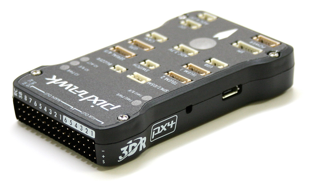
\includegraphics{hardware-pixhawk.png}
    \caption{Autopiloto Pixhawk}
    \label{fig:pixhawk1}
\end{figure}

El hardware autopiloto Pixhawk se puede programar con otro software distinto al del fabricante, entre aquellas soluciones las que son aplicables según las condiciones de diseño y de código abierto son ArduPilot, iNAV y Paparazzi, además del mismo PX4 \cite{survey}. Revisando a un poco más detalle cada alternativa se puede notar que, iNAV no ofrece opciones de vuelo autónomo avanzadas como aterrizaje automático, que serán de interés en el capítulo de diseño de algoritmos de control. Paparazzi es una opción bastante interesante que si tiene un sistema autónomo completo por medio de archivos ``XML'' con la información del plan de vuelo \cite{paparazzi_flight_plan}, pero no es compatible con el software de control en tierra utilizado por ArduPilot y PX4, siendo Mission Planner y QGroundControl los principales.

\begin{figure}[h]
    \centering
    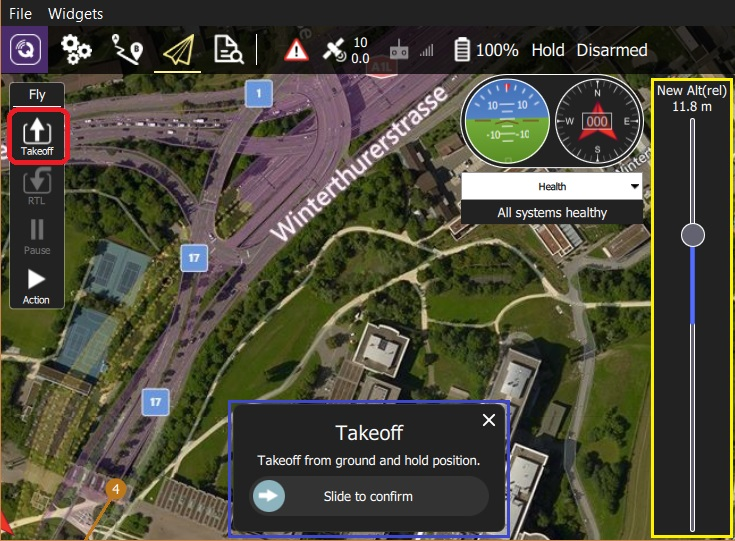
\includegraphics[width=0.7\textwidth]{takeoff.jpg}
    \caption{Software de estación en tierra QGroundControl}
    \label{fig:qgroundcontrol}
\end{figure}

PX4 es una opción atractiva ya que ofrece soporte para trabajar con técnicas ``Hardware-in-the-Loop'' con simuladores incluyendo X-Plane \cite{px4-hitl}. Sin embargo, aunque ArduPilot haya deprecado esa opción \cite{ap-hitl} existe más documentación en comparación con PX4 sobre como modificar existentes e implementar nuevos algoritmos de control \cite{ap-custom-controller}. Por esto último se decide en ArduPilot como plataforma de desarrollo.

\section{Extensión de protocolo de comunicación}

El protocolo de comunicación desarrollado durante el proyecto de ingeniería aeroespacial, inoFS, permite a X-Plane comunicarse con un microcontrolador. La interfaz disponible para lograrlo es aquella disponible en prácticamente todos los controladores, UART o mejor conocida como Serial sobre USB. Para microcontroladores que ofrezcan acceso a la red por wifi o Ethernet inoFS también puede trabajar con paquetes UDP.

\begin{figure}[h]
    \centering
    \includesvg[width=0.7\textwidth]{diagrama-fssp.svg}
    \caption{Funcionamiento inoFS}
    \label{fig:inofs-diagrama}
\end{figure}

Los detalles de su funcionamiento están en el informe de proyecto de ingeniería, pero cabe destacar el ``Programa intermediario'' en \cref{fig:inofs-diagrama} que es el principal responsable de traducir y reenviar los mensajes entre el simulador y el microcontrolador, se puede observar el programa funcionando junto a X-Plane en \cref{fig:inofs-programa-intermediario}.

\begin{figure}[h]
    \centering
    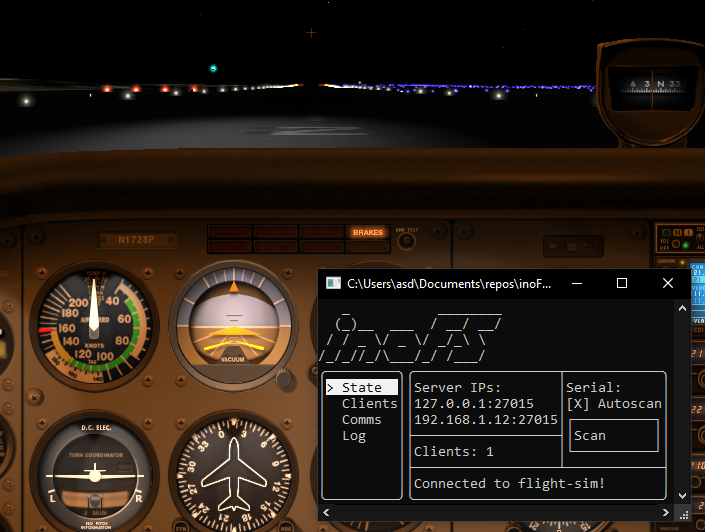
\includegraphics[width=0.6\textwidth]{inofs.png}
    \caption{Programa intermediario de inoFS}
    \label{fig:inofs-programa-intermediario}
\end{figure}

Para poder extender el protocolo de comunicación se debe ser capaz de realizar dos funciones, ingresar a ArduPilot el estado de vuelo de X-Plane como respuesta obtenida de sensores, y el ejecutar las acciones de control producidas por ArduPilot en X-Plane. Con estas funciones se puede considerar lista la implementación ``Processor-in-Loop'' y a continuación se describe el proceso para lograr cada una.

\subsection{Ingresar información de sensores a ArduPilot}

La primera opción a evaluar para poder entregarle a ArduPilot información de sensores es la descrita en la metodología en el capítulo 1, emular la misma respuesta que producirían sensores de verdad con algún microcontrolador y comunicarla por los puertos apropiados como son los de \cref{fig:pixhawk-ports}. Para sensores sencillos que producen una respuesta análoga como un potenciómetro esto es posible, pero los sensores utilizados en RPAS en su mayoría son digitales, por ejemplo los sensores en el Pixhawk disponible en el laboratorio son los siguientes \cite{pixhawk1}.

\begin{itemize}
    \item ST Micro L3GD20H 16 bit gyroscope
    \item ST Micro LSM303D 14 bit accelerometer / magnetometer
    \item Invensense MPU 6000 3-axis accelerometer / gyroscope
    \item MEAS MS5611 barometer
\end{itemize}

Todos son sensores digitales, esto significa que al iniciar el sistema se les entrega alguna opción de configuración con la ayuda de un driver, y luego estos responden con las lecturas en un formato específico para cada sensor en forma de paquetes discretos. Por ejemplo el giroscopio L3GD20H espera que el microcontrolador (en este caso el que esté programado con ArduPilot) haga lecturas a ubicaciones en memoria del giroscopio \cite{gyro-datasheet}. Una de las ubicaciones de memoria en el giroscopio contiene información de sí las lecturas se han visto saturadas o si hay un valor nuevo como se ve en \cref{fig:gyro-health}. Emular cada sensor a una suficiente fidelidad capaz de ``engañar'' a ArduPilot de que está recibiendo lecturas reales es demasiado trabajo, por lo que se decide buscar alternativas.

\begin{figure}[h]
    \centering
    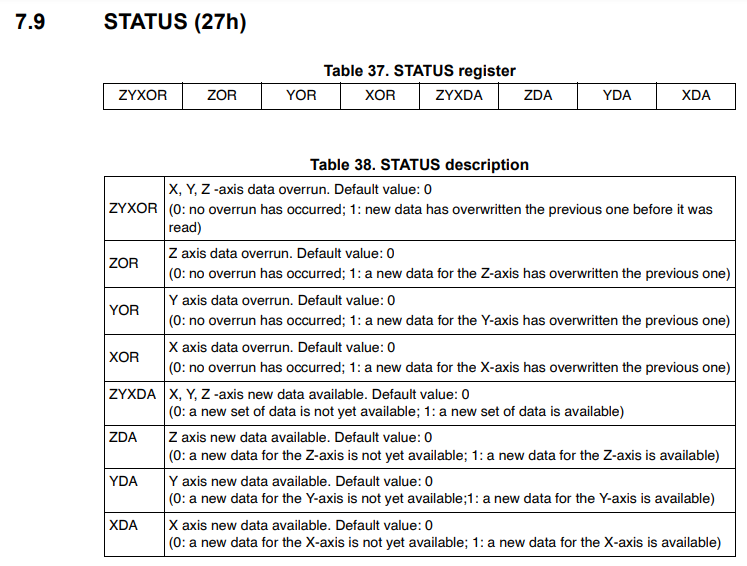
\includegraphics[width=0.6\textwidth]{gyro-registers.png}
    \caption{Ubicación en memoria del giroscopio con información de salud de las lecturas}
    \label{fig:gyro-health}
\end{figure}

El hardware autopiloto donde puede funcionar ArduPilot (como es el Pixhawk disponible en el laboratorio) incluye puertos Serial disponibles para muchas funciones como son el recibir lecturas de sensores que trabajen con esa interfaz, enviar y recibir mensajes que utilizan el protocolo de telemetría MavLink \cite{ap-serial} o para alguna aplicación personalizada que el usuario quisiera programar por medio de scripting en el lenguaje Lua \cite{ap-scripting}.

\begin{figure}[h]
    \centering
    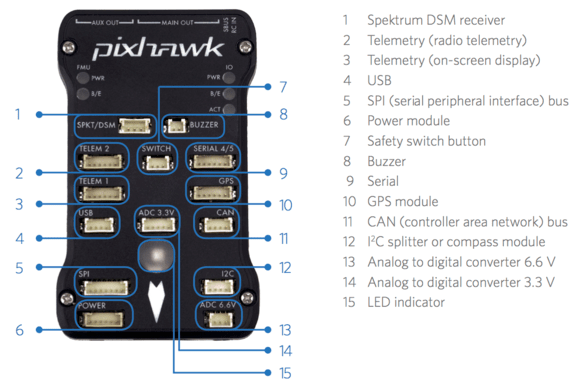
\includegraphics[width=0.6\textwidth]{pixhawk-ports.png}
    \caption{Puertos en Pixhawk}
    \label{fig:pixhawk-ports}
\end{figure}

La siguiente alternativa evaluada es enviar lecturas de sensores generadas con algún protocolo propio por alguno de los puertos Serial, y programar ArduPilot para que las interprete como lecturas de un sensor personalizado. Esto último es difícil, porque se debe de alguna forma programar ArduPilot.

Primero se consideró aprovechar el motor de scripting en Lua para esta tarea. La ventaja de utilizar scripts es que no necesita modificar el código fuente de ArduPilot y por lo tanto tampoco reprogramar por completo el microcontrolador del autopiloto, ya que los scripts se cargan de manera dinámica desde la tarjeta SD. Lamentablemente los scripts no cuentan con la funcionalidad de poder generar lecturas de sensores críticos como son el IMU o GPS por lo que se descarta esta opción.

Estudiando el código fuente de ArduPilot se identificó que este soporta sistemas de estimación de actitud externos o ``External Attitude Heading Reference System'', están compuestos por una combinación de sensores y un procesador que realiza su propia fusión exportando un cuaternión describiendo la actitud junto con posición y velocidad en un marco de referencia inercial. Actualmente ArduPilot soporta tres sistemas de estimación de actitud externos disponibles en el mercado \cite{ap-eahrs}.

\begin{itemize}
    \item MicroStrain 3DM® Series
    \item VectorNav VN-300 AHRS
    \item VectorNav VN-100 AHRS
\end{itemize}

ArduPilot ofrece la opción de utilizar la estimación de actitud producida por el sistema externo directamente, o de forma alternativa solo recibir las mediciones de los sensores y por medio de un filtro de Kalman generar su propia estimación. En el contexto del proyecto ambas opciones son útiles, el que ArduPilot reciba la información de actitud perfecta de X-Plane permite descartar esta variable de los problemas que se vayan a producir durante las pruebas del controlador personalizado. Y el solo incorporar las lecturas de sensores y que ArduPilot realice su propia estimación con filtro de Kalman es lo que este haría en un vuelo real.

Se decidió escribir un driver para un nuevo sistema de estimación de actitud externo ficticio el cual recibirá lecturas de sensor y actitud por medio de conexión Serial, que además entregara por esta misma conexión la respuesta de la acción de control que esté produciendo ArduPilot como salidas de servo. La creación de este nuevo driver en el lado de ArduPilot implica que se debe modificar el código fuente, en \cref{fig:eahrs} se pueden observar los archivos que componen los sistemas de estimación de actitud externos, la clase principal \texttt{AP\_ExternalAHRS} y la implementación de los sistemas ``MicroStrain'' y ``VectorNav'', en los archivos \texttt{AP\_ExternalAHRS\_MicroStrain5} y \texttt{AP\_ExternalAHRS\_VectorNav}. El código fuente del nuevo driver se escribió en los archivos \texttt{AP\_ExternalAHRS\_HITL}, hasta este punto con la implementación más básica que lograse compilar y ser cargada en un autopiloto de pruebas.

\begin{figure}[h]
    \centering
    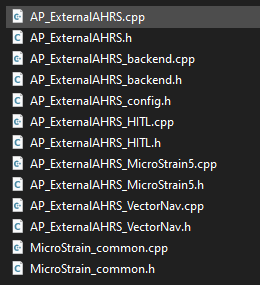
\includegraphics[width=0.3\textwidth]{eahrs.png}
    \caption{Archivos de código fuente para sistemas de estimación de actitud externos}
    \label{fig:eahrs}
\end{figure}

El proceso de compilación de ArduPilot está documentado \cite{ap-build} y se puede cargar al autopiloto por USB de la misma forma que actualizando firmware de ArduPilot oficial. En el laboratorio de técnicas aeroespaciales se proporcionó de un autopiloto PixHawk 4 soportado de manera oficial por los desarrolladores de ArduPilot \cite{pixhawk4}. Para realizar la modificación del firmware de manera ordenada se creó un ``fork'' de la versión estable de ArduPlane en el momento de escritura del informe 4.4.2, sobre la que se escribe el nuevo driver y se lleva un registro de cada cambio en el repositorio en GitHub \cite{ap-hitl-fork}.

Una vez cargado ArduPilot modificado, con el programa de estación en tierra Mission Planner se ajusta el parámetro que indica que se utilizara un sistema inercial externo como se puede observar en \cref{fig:missionplanner-params}. Mission Planner no reconoce el nombre de la nueva opción correctamente mostrando un espacio en blanco, pero al seleccionarla y reiniciar el autopiloto se puede comprobar que se está ejecutando el nuevo driver observando el registro como se ve en \cref{fig:missionplanner-log}.

\begin{figure}[h]
    \centering
    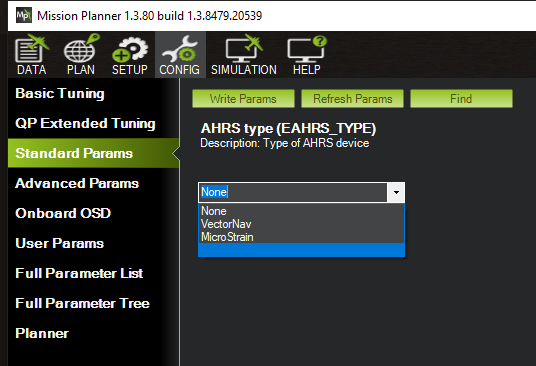
\includegraphics[width=0.6\textwidth]{missionplanner-params.png}
    \caption{Selección de sistema inercial externo en Mission Planner}
    \label{fig:missionplanner-params}
\end{figure}

\begin{figure}[h]
    \centering
    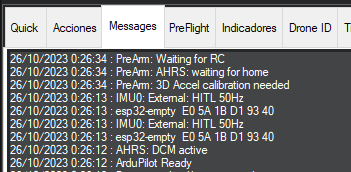
\includegraphics[width=0.4\textwidth]{missionplanner-log.png}
    \caption{Registro de inicialización de Mission Planner}
    \label{fig:missionplanner-log}
\end{figure}

Durante las pruebas se descubrió un nuevo posible problema, como ha sido descrito hasta ahora se busca extender el protocolo de comunicación creado en el proyecto de ingeniería, inoFS. Sin embargo existe una limitación producto de su diseño. inoFS en sí extiende FSUIPC, el cual es un plug-in para Microsoft Flight Simulator que permite lectura y escritura arbitraria de variables internas del simulador, XPUIPC es una reimplementación del plug-in compatible con X-Plane que trabaja de la misma forma que FSUIPC. El problema es que la frecuencia a la que FSUIPC o XPUIPC pueden leer información de la simulación no está definida, y los sensores encontrados en los autopilotos pueden llegar a entregar lecturas a una frecuencia de hasta 1000 Hz como lo hace el MPU-6000. Además de la incerteza de la velocidad de FSUIPC está la latencia producto de tener que enviar la información a través del programa intermediario. Para asegurar la máxima frecuencia de datos posible se decidió no utilizar inoFS, y en su lugar crear un plug-in específico para X-Plane que envíe información por puerto Serial directo luego de cada paso de la simulación, eliminando cualquier retraso posible en el canal de comunicación. Se lleva registro del desarrollo del plug-in en un repositorio en GitHub de la misma manera que para el ``fork'' de ArduPilot \cite{xplane-hitl-plugin}.

\begin{figure}[h]
    \centering
    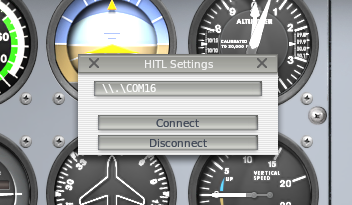
\includegraphics[width=0.4\textwidth]{hitl-plugin-1.png}
    \caption{Primera versión de plug-in ``PIL'' para X-Plane}
    \label{fig:hitl-plugin-1}
\end{figure}

El puerto serial al que el plug-in de X-Plane envía los datos no es el del autopiloto, en un computador se accede a puerto serial por USB y los sistemas inerciales externos no son USB, sino que utilizan dos pines ``RX'' y ``TX'' de entrada y salida. Por esto para completar la implementación del sistema inercial externo ficticio se utiliza otro microcontrolador que reenviara los mensajes desde X-Plane hasta el autopiloto y viceversa, como se visualiza en \cref{fig:plugin}. En este caso se utiliza una Raspberry Pi Pico donde se configuran dos interfaces serial, una por USB y otra por los pines GPIO 4 y 5 ubicados como se ve en \cref{fig:pico-pins}. El puerto serial que utilizara el autopiloto se configura en los parámetros accesibles en Mission Planner como se ve en \cref{{fig:missionplanner-params-serial}}, donde ``Serial 2'' hace referencia al puerto serial 2 que está en cada autopiloto asignado a ciertos pines indicados por alguna etiqueta en la carcasa, como se puede observar en el Pixhawk en \cref{fig:pixhawk-ports} donde seria ``Telem 2''.

\begin{figure}[h]
    \centering
    \includesvg[width=0.7\textwidth]{plugin.svg}
    \caption{Comunicación entre X-Plane y autopiloto}
    \label{fig:plugin}
\end{figure}

\begin{figure}[h]
    \centering
    \includesvg[width=0.5\textwidth]{pico-pins.svg}
    \caption{Diagrama de pines en Raspberry Pi Pico}
    \label{fig:pico-pins}
\end{figure}

\begin{figure}[h]
    \centering
    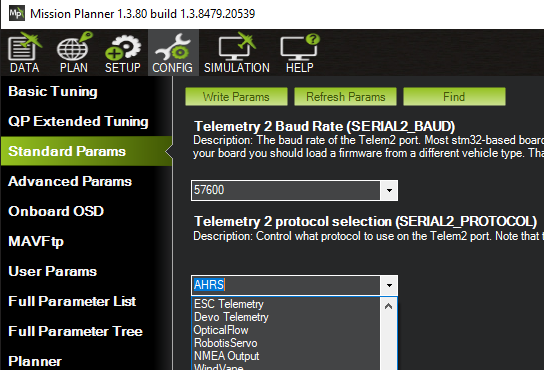
\includegraphics[width=0.6\textwidth]{missionplanner-params-serial.png}
    \caption{Especificación de función de puerto serial en Mission Planner}
    \label{fig:missionplanner-params-serial}
\end{figure}

Con todo configurado y conectado como en \cref{fig:setup} se logra comprobar que la información de X-Plane está siendo procesada por el autopiloto, en \cref{fig:qgroundcontrol} se observa que los movimientos del horizonte artificial del software en tierra (ahora QGroundControl) corresponden al de la inclinación de la aeronave. Hasta este punto se nota que el horizonte esta al revés porque aún falta procesar y calibrar un poco los datos para entregarlos de la forma que espera ArduPilot y no utilizar valores directos desde X-Plane.

\begin{figure}[h]
    \centering
    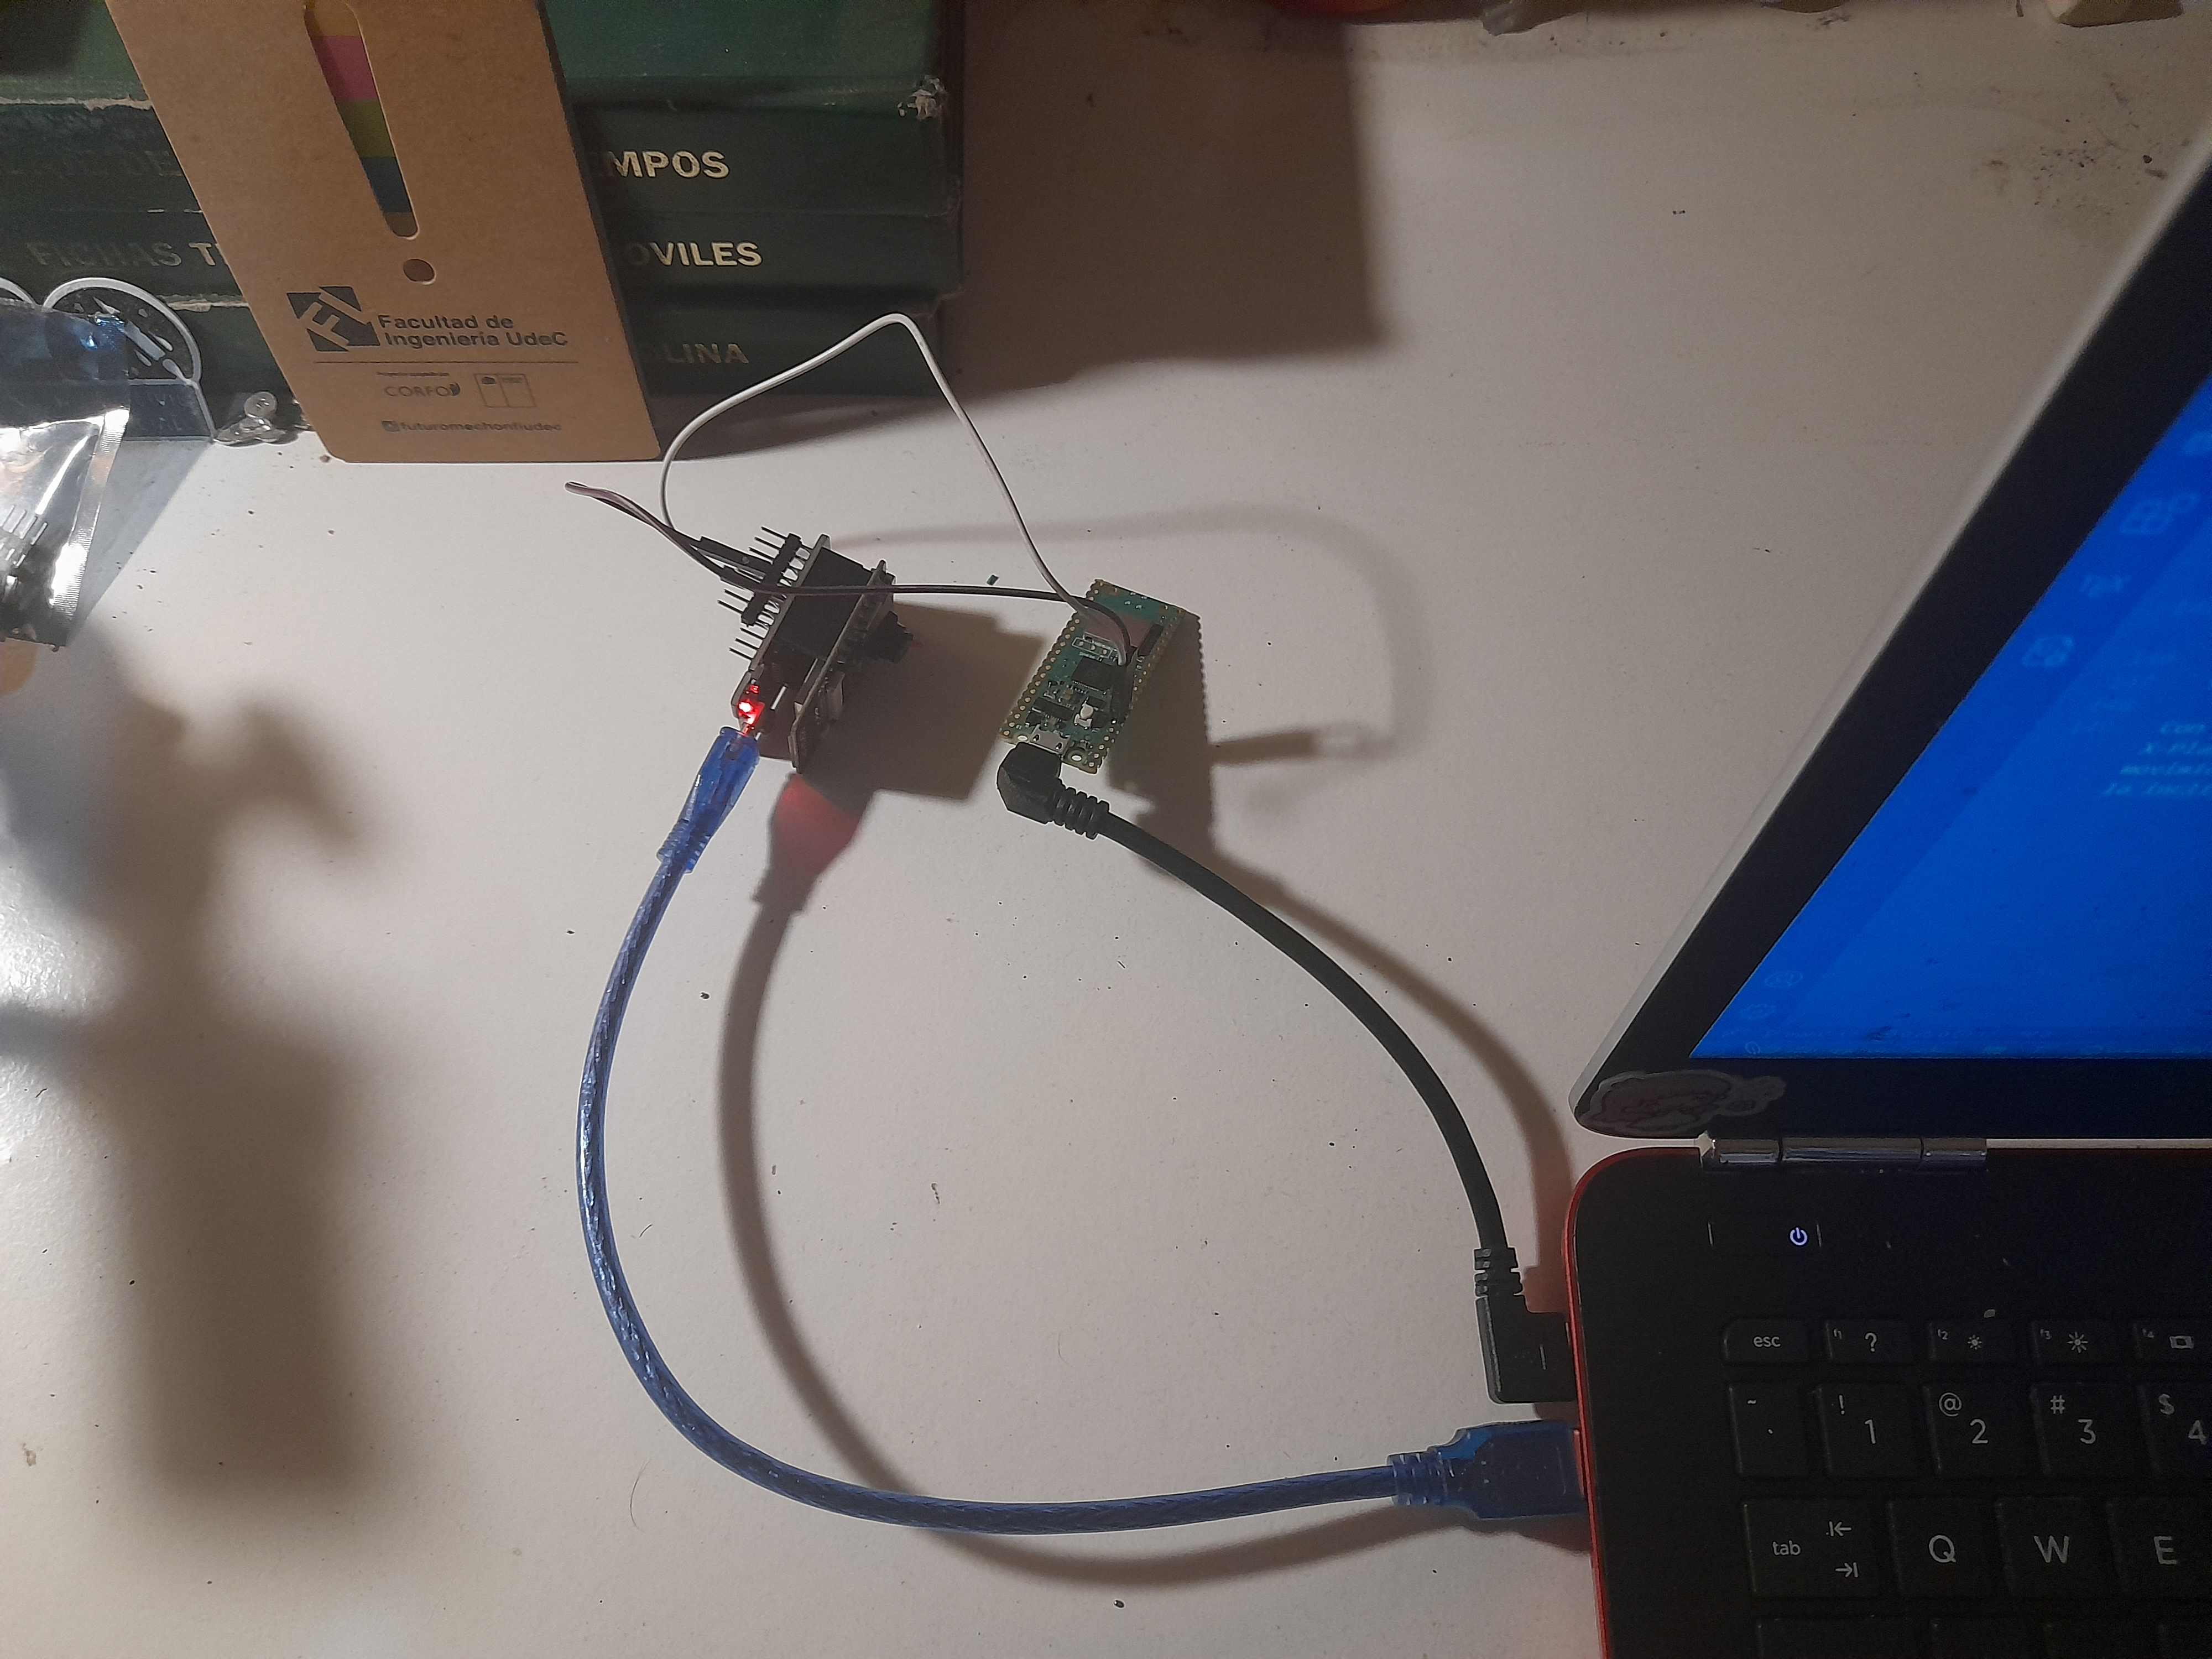
\includegraphics[width=0.6\textwidth]{setup.jpg}
    \caption{Autopiloto y microcontrolador comunicados por dos cables serial}
    \label{fig:setup}
\end{figure}

\begin{figure}[h]
    \centering
    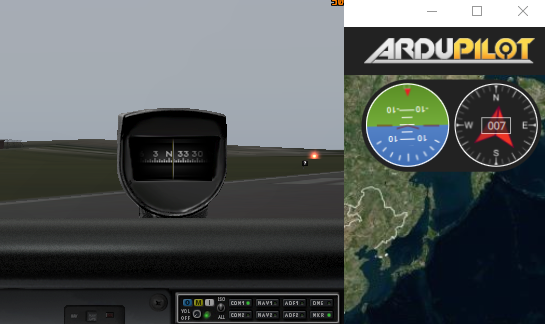
\includegraphics[width=0.6\textwidth]{xplane-qgroundcontrol.png}
    \caption{Lecturas de inclinación y orientación en QGroundControl}
    \label{fig:qgroundcontrol}
\end{figure}

\subsection{Ejecución de acciones de control en X-Plane}

[todo]